%
% CHAPTER 1.- Preliminaries
%

\chapterimage{Koenigsberg_Map_by_Bering_1613.pdf} % Chapter heading image

\chapter{Discrete Mathematics}
\label{chap:Discrete_Mathematics}

\begin{quote}
\begin{flushright}
\emph{Mathematics may be defined as the subject in which\\
we never know what we are talking about,\\
nor whether what we are saying is true.}\\
Bertrand Russell
\end{flushright}
\end{quote}
\bigskip

Most of the mathematics used throughout this book belong to the area of \emph{discrete mathematics}. Discrete mathematics is characterized because it studies mathematical objects that have distinct or separated values, rather than continuous. Examples of discrete objects used in this book are integers, strings, graphs and computer programs. A key distinctive element of discrete sets is that they can be enumerated with natural numbers, that is, they are countable. We will barely use continuous mathematics, for example calculus, in the theoretical developments of the theory of nescience.

Our main interest in discrete mathematics is because computers. The theory of nescience borrows concepts and ideas from multiple areas of computer science: algorithms, coding, string complexity and others. Computers operate in discrete steps and the data processed is stored in discrete units of memory. We are interested in computers because we want to apply our theoretical developments to as many real objects as possible, and we think that the right way to model our world is by means of using computers. In pure mathematics it is customary to discuss abstract objects without worrying about what they represent. In the theory of nescience, on the contrary, the representation (encoding) of objects plays a crucial role.

This chapter is intended as a quick review of the basic concepts of discrete mathematics; no formal definitions are provided and theorems are not proved. Discrete mathematics is an extremely diverse and large area of study. We will review only those elements that are required to understand the theory of nescience. Some of the theories involved (computability, information, complexity, ...) require a deeper coverage, and so, they are studied in separate chapters. In the References section there is a list of suggested books that explain in detail the topics covered in this chapter.

%
% Section: Strings
%

\section{Strings}
\label{sec:strings}

Let $\mathcal{S}=\left\{ s_{1},s_{2},\ldots,s_{q}\right\}$ be a non-empty finite set called \emph{alphabet}\index{Alphabet}. A \emph{sequence} over $\mathcal{S}$ is any ordered collection of symbols $x_1 x_2 \dots x_n$ from $\mathcal{S}$. When the alphabet is the set $\mathcal{B} = \{0, 1\}$, the sequences are called \emph{binary}. If the sequence is finite we call it \emph{string}\index{string}. In this book we will be working most of the time with binary strings. The \emph{length}\index{Length of a string} of a string $s$, denoted by $l(s)$, is the number of symbols in $s$. The \emph{empty string}\index{Empty string} is the unique string over $\mathcal{S}$ of length 0, and is denoted $\lambda$. Let $x \in \mathcal{S}$, by $x^n$ we denote the string $x x \ldots x$ ($n$-times). If $s = x_1 x_2 \dots x_n$ is a string, its \emph{reverse}\index{Reverse string} $s^R$ is $x_n x_{n-1} \dots x_1$.

Let $\mathcal{S}^{n}$ denote the set of all strings $s_{1}s_{2}\ldots s_{n}$ of length $n$\footnote{Do not confuse the set of strings of length $n$ over an alphabet $\mathcal{S}^n$ with the $n$-fold Cartesian product of a set $S^n$, alphabets will be represented by using calligraphic fonts.}, $\mathcal{S}^{+}=\cup_{n\geq1}\mathcal{S}^{n}$ and $\mathcal{S}^{\ast} = \mathcal{S}^{+} \cup \{\lambda\}$. Note that all the strings that belong to $\mathcal{S}^{\ast}$ have finite lengths.

\begin{example}
The following relations hold: $d \left( \left\{ s \in \mathcal{B}^{\ast} : l(s) = n \right\} \right) = 2^n$ and $d \left( \left\{ s \in \mathcal{B}^{\ast} : l(s) \leq n \right\} \right) = 2^{n+1}-1$.
\end{example}

For any two strings $s$ and $t$ in $\mathcal{S}^{\ast}$, the \emph{concatenation}\index{String concatenation} of $s$ and $t$, denoted by $st$, is defined as the sequence of symbols in $s$ followed by the sequence of symbols in $t$. Note note that $l(st) = l(s) + l(t)$. $S^\ast$ is closed under the operation of concatenation. $S^\ast$ with the operation of concatenation forms a \emph{free monoid}, that it, it is associative  $s(tr)=(st)r$, and has an identity element $\lambda a = a \lambda = a$.

A string $s$ is said to be a \emph{substring}\index{Substring} of $t$ if there exist (possibly empty) strings $u$ and $v$ such that $t$ = $usv$. A string $s$ is said to be a \emph{prefix}\index{Prefix} of $t$, denoted by $s <_p t$, if there exists a string $u$ such that $t = su$. A subset $S \subset \mathcal{S}^{\ast}$ is \emph{prefix free}\index{Prefix free set} if for all $s, t \in S$, if $s <_p t$ then $s = t$. Given a string $s \in \mathcal{S}^{\ast}$, the \emph{self delimited}\index{Self delimited string} version of $s$, denoted by $\bar{s}$, is $\bar{s} = 1^{l(s)}0s$. Note that $l(\bar{s}) = 2l(s)+1$.

\begin{example}
The set $\bar{\mathcal{S}^{\ast}}$composed by all the self delimited strings of $\mathcal{S}^{\ast}$ is prefix free.
\end{example}

If $\mathcal{S}$ is a total ordered set, we can define a total order on $\mathcal{S}^{\ast}$, called \emph{shortlex ordering}\index{Shortlex ordering}, in which sequences are primarily sorted by length with the shortest sequences first, and sequences of the same length are sorted into their lexicographical order.

\begin{example}
If $S = \{a, b, c\}$ and $a < b < c$, then the shortlex order on $\mathcal{S}^{\ast}$ includes the relations $\lambda < a < b < c < aa < ab < \ldots < cc < aaa < aab < \ldots < ccc < \ldots$
\end{example}

Given an arbitrary object $O$ we denote its representation as a string as $\left\langle O\right\rangle$, assuming that there exists an standard encoding method. Given the objects $O_{1},O_{2},\ldots,O_{k}$, the concatenation of the representations of these objects $\left\langle O_1 \right\rangle \left\langle O_2 \right\rangle \ldots \left\langle O_k \right\rangle$ is denoted by $\left\langle O_1 O_2 \ldots O_k \right\rangle$. The concatenation of the representation of these objects in such a way that we can decode and uniquely identify all of them is represented by $\left\langle O_1, O_2,\ldots,O_k \right\rangle$, for example, we could use $\left\langle O_1, O_2,\ldots,O_k \right\rangle = \bar{\left\langle O_1 \right\rangle} \bar{\left\langle O_2 \right\rangle} \ldots \bar{\left\langle O_k \right\rangle}$.

\begin{example}
Natural numbers can be represented by binary strings using the following encoding method: $\langle 0 \rangle = \lambda$, $\langle 1 \rangle \rightarrow 0$, $\langle 2 \rangle \rightarrow 1$, $\langle 3 \rangle \rightarrow 00$, $\langle 4 \rangle \rightarrow 01$, $\langle 5 \rangle \rightarrow 10$, $\langle 6 \rangle \rightarrow 11$, $7 \rightarrow 000$, ... For example $\left\langle 3, 7 \right\rangle$  would be represented as $110001110000$. Given this encoding we have that $l \left( \langle n \rangle \right) = \lfloor \log_2 (n + 1) \rfloor$.
\end{example}

{\color{red} TODO: Introduce the Kleene closure and free monoids.}

%
% Section: Matrices
%

\section{Matrices}
\label{sec:preliminaries-matrices}

A \emph{matrix} $A$ of order $m \times n$ is a set of $mn$ scalars ordered in $m$ \emph{rows} and $n$ \emph{colums} in the following way:
\[
A = 
 \begin{pmatrix}
  a_{1,1} & a_{1,2} & \cdots & a_{1,n} \\
  a_{2,1} & a_{2,2} & \cdots & a_{2,n} \\
  \vdots  & \vdots  & \ddots & \vdots  \\
  a_{m,1} & a_{m,2} & \cdots & a_{m,n} 
 \end{pmatrix}
\]
The \emph{entry} $a_{ij}$ corresponds to the element of $A$ localed at row $i$ and column $j$. We denote by $\mathcal{M}_{m \times n}$ the \emph{set of all matrices} of order $m \times n$. A \emph{row matrix} is a matrix that belongs to $\mathcal{M}_{1 \times n}$, and a \emph{column matrix} to $\mathcal{M}_{m \times 1}$. A \emph{squared matrix} is a matrix that belongs to $\mathcal{M}_{n \times n}$. The entries $a_{ii}$ form the \emph{main diagonal} of a square matrix. The \emph{transpose matrix} of a matrix $A \in \mathcal{M}_{m \times n}$ is the matrix $A^T \in \mathcal{M}_{n \times m}$ whose entries $(i,j)$ are equal to the entries $(j, i)$ of $A$. If $A = A^T$ we say that $A$ is a \emph{symmetric matrix}. A \emph{diagonal matrix} is a matrix whose all its entries outside the main diagonal are zero. The \emph{identity matrix} $I$ is a diagonal squared matrix with all the entries in the main diagonal equal to 1. A \emph{submatrix} of a matrix is obtained by deleting any collection of rows and/or columns.

\begin{example}
Given the squared matrix $A = \left( \begin{smallmatrix} 1 & 2 & 3 \\ 4 & 5 & 6 \\ 7 & 8 & 9 \end{smallmatrix} \right)$ we have that the entry $(2, 3)$ has the value $6$, the diagonal is composed by the numbers $1$, $5$, and $9$, its transpose is $A^T = \left( \begin{smallmatrix} 1 & 4 & 7 \\ 2 & 5 & 8 \\ 3 & 6 & 9 \end{smallmatrix} \right)$, and that the matrix $B = \left( \begin{smallmatrix} 1 & 3 \\ 4 & 6 \end{smallmatrix} \right)$ is a submatrix of $A$.
\end{example}

The sum of two matrices $A$ and $B$ of equal size is the matrix $A + B$ whose entry $(i, j)$ are $(A + B)_{ij} = a_{ij} + b_{ij}$. The operation of sum of matrices is associative $(A + B) + C = A + (B + C)$, commutative $A + B = B + A$, has a neutral element $A + 0_{m \times n} = A$ and an inverse element $A + (-A) = 0_{m \times n}$. The multiplication of a scalar $\lambda$ by a matrix $A$ is the matrix $\lambda A$ whose entry $(i, j)$ is $(\lambda A)_{ij} = \lambda a_{ij}$. The operation of multiplication of a scalar by a matrix is distributive with respect to the sum of matrices $\alpha (A + B) = \alpha A + \alpha B$, distributive with respect to the sum of scalars $(\alpha + \beta) A = \alpha A + \beta B$, associative with respect to the product by scalars $(\alpha \beta) A = \alpha (\beta A)$, and has a unit element $1 A = A$. The product of two matrices $A_{m \times n}$ and $B_{n \times p}$ is the matrix $AB_{m \times p}$ whose entry $(i, j)$ is $(AB)_{ij} = \sum_{k=1}^n a_{ik} b_{kj}$. The operation of multiplication of matrices os associative $(A B) D = A (B D)$, has a left neutral element $A I_n = A$ and a right neutral element $I_m A = A$, associative with respect to the product by scalars $\alpha (A B) = (\alpha A) B = A (\alpha B)$, distributive with respect the sum of matrices by the right $A (B + C) = AB + AC$ and the left $(B + C) D = B D + C D$. Additionally, the operation of traspose satisfies the following properties: $(A + B)^T = A^T + B^T$, $(\lambda A)^T = \lambda A^T$, $(A B)^T = B^T A^T$.

\begin{example}
Given the matrices $A = \left( \begin{smallmatrix} 1 & 2 \\ 3 & 5 \end{smallmatrix} \right)$ and $B = \left( \begin{smallmatrix} 5 & 6 \\ 7 & 8 \end{smallmatrix} \right)$ we have that $A + B = \left( \begin{smallmatrix} 6 & 8 \\ 10 & 13 \end{smallmatrix} \right)$, $2 A = \left( \begin{smallmatrix} 2 & 4 \\ 6 & 10 \end{smallmatrix} \right)$ and $A B = \left( \begin{smallmatrix} 19 & 22 \\ 50 & 58 \end{smallmatrix} \right)$.
\end{example}


%
% Section: Graphs
%

\section{Graphs}
\label{sec:Graphs}

A \emph{graph}\index{Graph}\footnote{The definition of graph provided in this introduction is equivalent to the definition of \emph{simple graph} in the standard discrete mathematics literature.} $G$ is an ordered pair $(V,E)$ composed by a nonempty set of objects $V$, called \emph{vertices}\index{Vertices of a graph}, connected by set of links $E$, called \emph{edges}\index{Edges of a graph}. The elements of $E$ have the form of unordered pairs $\left\{ u,v\right\}$ of distinct (no loops allowed) vertices $u$,$v\in V$. Vertices $u$ and $v$ are said to be \emph{adjacent}\index{Adjacent vertices} if there is and edge $\left\{ u,v\right\} \in E$, and if so, they are called the \emph{endpoints}\index{Endpoints of an edge} of the edge. If the set $V$ is infinite, the graph is called \emph{infinite graph}\index{Infinite graph}; however, in this book we will consider only finite graphs. If the pairs of vertices $u, v$ are ordered pairs, the graph is called \emph{directed graph}\index{Directed graph}, and in that case, $u$ is called the \emph{initial vertex}\index{Initial vertex} and $v$ the \emph{terminal vertex}\index{Terminal vertex}. If $G = (V,E)$ is a graph, its \emph{adjacency matrix}\index{Adjacency matrix} is a square $d(V) \times d(V)$ matrix $A$ such that the element $A_{uv}$ is 1 if $\left\{ u,v\right\} \in E$ and 0 otherwise.

Graphs are usually depicted as a set of dots for the vertices, joined by lines for the edges. If the graph is directed, we use arrows instead of lines to represent edges.

\begin{example}
Let $V=\{a, b, c, d\}$ and $E=\{ \{a,b\}, \{a,c\}, \{a,d\}, \{b,c\} \}$, the graph $G=(V,E)$ is depicted in Figure \ref{fig:Graph-Example}.
\end{example}

\begin{figure}[h]
\centering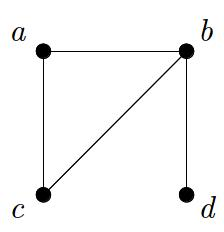
\includegraphics[scale=0.5]{GraphExample}
\caption{\label{fig:Graph-Example}An Example of Graph}
\end{figure}

If $v$ is an endpoint of and edge $e$, then we say that $e$ is is \emph{incident}\index{Incident edge} on $v$. The \emph{degree}\index{Degree of a vertex} of a vertex $v$, written $\deg(v)$, is equal to the number of edges which are incident on $v$. A vertex of degree zero is called \emph{isolated}\index{Isolated vertex}; a vertex of degree one is called \emph{pendant}\index{Pendant vertex}. The \emph{neighborhood}\index{Neighborhood of a vertex} of vertex $v$, denoted by $N(v)$, is the set of all vertices that are adjacent to $v$. If $A \subset V$, the neighborhood of $A$ is $N(A) = \cup_{v \in A} N(v)$. If $G$ is directed graph, we call the \emph{in-degree}\index{In-degree of a vertex} of a vertex $v$, denoted by $indeg(v)$, to the number of edges in which $v$ is an terminal vertex, and \emph{out-degree}\index{Out-degree of a vertex}, denoted by $outdeg(v)$, to the number of edges in which $v$ is an initial vertex. A \emph{path}\index{Path} in a graph is a sequence of distinct vertices $\{v_{0}, v_{1}, \ldots ,v_{k}\}$ in which $v_{i}$ and $v_{i+1}$ are adjacent for each $1 \leq i < k$. If $v_{0} = v_{k}$ we say that the path is a \emph{cycle}\index{Cycle}.

\begin{example}
Given a graph $G=(V,E)$, the \emph{handshaking theorem}\index{Handshaking theorem} states that $\sum_{v \in V} deg(v) = 2 m$, where $m = d(E)$, since each edge has two end points.
\end{example}

A graph $G$ is said to be \emph{bipartite}\index{Bipartite graph} if the set of vertices $V$ can be partitioned into two subsets $V_1$ and $V_2$ such that each edge of $G$ connects a vertex of $V_1$ to a vertex of $V_2$. Bipartite graphs are usually denoted by $G=(V_1, V_2, E)$. The degree of the vertices of a bipartite graph satisfied the following property, called the \emph{degree sum formula}\index{Degree sum formula}, $\sum_{u \in V_1} deg(u) = \sum_{v \in V_2} deg(v) = d(E)$.

A graph $G(V',E')$ is a \emph{subgraph}\index{Subgraph} of $G(V,E)$ if $V'$ is a subset of $V$ and $E'$ is a subset of $E$ whose endpoints belong to $V'$. A graph $G$ is called a \emph{labeled graph}\index{Labeled graph} if its edges and/or vertices are assigned data of one kind or another. In particular, if each edge $e$ of $G$ is assigned a nonnegative number $w(e)$ then $w(e)$ is called the \emph{weight}\index{Weight of an edge} of $e$.

A particular type of graph that will be extensively used in this book are trees. A \emph{tree}\index{Tree} is a non-empty graph in which any two vertices are connected by a unique path. Given a tree, we will always designate a particular vertex, called the \emph{root}\index{Root of a tree} of the tree, and direct each edge away from that root.

\begin{example}
An equivalent definition of trees is provided by set theory. According to set theory a tree is a partially ordered set $(T, <)$ such that for each $t \in T$, the set $S = \{ s \in T : s < t \}$ has an element that is smaller than every other element of S (\emph{least element}).
\end{example}

Let $T$ be a tree. If $v$ is a vertex in $T$ other than the root, the \emph{parent}\index{Parent of a vertex} of $v$ is the unique vertex $u$ such that there is an edge connecting $u$ to $v$. If $u$ is the parent of $v$, then $v$ is called a \emph{child}\index{Child of a vertex} of $u$. A \emph{sibling}\index{Sibling to a vertex} to a vertex $v$ is any other vertex on the tree which has the same parent than $v$. The \emph{ancestors}\index{Ancestors of a vertex} of a vertex are the vertices in the path from the root to this vertex, excluding the vertex itself and including the root. The \emph{descendants}\index{Descendant of a vertex} of a vertex $v$ are those vertices that have $v$ as an ancestor. A vertex is called a \emph{leaf}\index{Leaf vertex} if it has no children. Vertices that have children are called \emph{branches}\index{Branches of a tree}. The \emph{depth}\index{Depth of a vertex} of a vertex $v$ is the length of the unique path from the root to $v$. The \emph{height}\index{Height of a tree} of a tree is the maximum of the levels of its vertices. 

\begin{example}
The following applies to the tree depicted in Figure \ref{fig:BinaryTree-Example}: the root is the vertex $a$; $c$ is a parent of $d$ and $d$ is a child of $c$; $d$ and $g$ are siblings; the ancestors of $d$ are $a$ and $c$; the descendants of $c$ are $e$, $e$ and $f$; $b$, $e$, $f$ and $g$ are leaf nodes; $c$ and $d$ are branches; the depth of $d$ is 3; the height of the tree is 4.
\end{example}

\begin{figure}[h]
\centering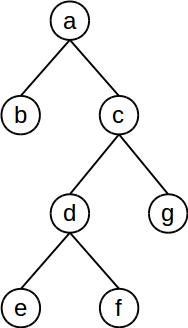
\includegraphics[scale=0.5]{BinaryTree}
\caption{\label{fig:BinaryTree-Example}An Example of Tree}
\end{figure}

If $v$ is a vertex in a tree, the \emph{subtree}\index{Subtree} with $v$ as root is the subgraph of the tree consisting of $v$ and its descendants and all edges incident to these descendants. A tree is called an \emph{k-ary tree}\index{k-ary tree} if every branch has not more than $k$ children. The tree is called a \emph{full k-ary tree}\index{full k-ary tree} if every branch has exactly $k$ children. An \emph{k-ary} tree with $k=2$ is called a \emph{binary tree}\index{Binary tree}. A $k$-ary tree of height $h$ is \emph{balanced}\index{Balanced tree} if all its leaves are have a depth of $h$ or $h-1$.

\begin{example}
A tree with $n$ vertices has $n-1$ edges. A full $k$-ary tree with $i$ branches contains $m=ki+1$ vertices.
\end{example}

{\color{red} TODO: Breadth first traversal}
{\color{red} TODO: Somewhere I should describe what it is a greedy algorithm}

%
% Section: Discrete Probability
%

\section{Calculus of Probability}
\label{sec:probability}

{\color{red} TODO: Include a note about the lack of a valid interpretation of the concept of probability, and why the axioms do not fit in the requirements of model theory.}

As we have said in the introduction of this chapter, our main interest is in discrete mathematics, and so, we will only provide a definition of probability for the case of discrete sets.

Let $\Omega$ be a finite or countable set, called \emph{sample space}\index{Sample space}, whose elements are called \emph{oucomes}\index{Outcome}. An \emph{event}\index{Event} $A$ is any subset of $\Omega$. We call $\Omega$ the \emph{certain event} and $\varnothing$ the \emph{impossible event}. We are only interested those collections of events $\mathcal{A} \subseteq \mathcal{P}\left( \Omega \right)$ that statisfy the following conditions: i) $\Omega \in \mathcal{A}$, ii) if $A \in \mathcal{A}$ then $A^c \in \mathcal{A}$, iii) if $A_1, A_2, \ldots$ be a countable collection of events of $\mathcal{A}$, then $\cup_{i=1}^\infty A_i \in \mathcal{A}$. Given these conditions we have that the impossible event is an event $\varnothing \in \mathcal{A}$, the union of a finite collection of events $A_1, A_2, \ldots, A_n \in \mathcal{A}$ is an event $A_1 \cup A_2 \cup \ldots \cup A_n \in \mathcal{A}$, and by applying De Morgan's laws, that the intersection of a fine or countable collection of sets of $\mathcal{A}$ is also in $\mathcal{A}$.

A \emph{probability}\index{Probability} is a number $P(A) \in \mathbb{R}$ assigned to each event $A \in \mathcal{A}$, that statisfy the following axioms:

\begin{description}

\item [Axiom 1] $P(A) \geq 0$.

\item [Axiom 2] $P(\Omega) = 1$.

\item [Axiom 3] For every infinite sequence of disjoint events $A_1, A_2, \ldots$ we have that $P(\cup_{i=1}^\infty A_i) = \sum_{i=1}^\infty P(A_i)$.

\end{description}

Probability is a number between $0$ and $1$. The probability of the impossible event $\varnothing$ is $0$. The probability of the complement event is $P(A^c) = 1 - P(A)$. If $A \subseteq B$ then we have that $P(A) \leq P(B)$. If $A$ and $B$ are not mutually exclusive then we have that $P(A \cup B) = P(A) + P(B) - P(A \cap B)$. The probability of a finite sequence of disjoint events $A_1, A_2, \ldots, A_n$ is $P(\cup_{i=1}^n A_i) = \sum_{i=1}^n P(A_i)$.

\begin{example}
Let $\Omega$ a sample space containing $n$ elements equally probable. If $A \subset \Omega$ is an event with $d(A) = m$, the we have that $P(A) = m/n$.
\end{example}

The \emph{conditional probability}\index{Conditional probability} of an event $A$ given the occurrence of another event $B$, is defined by $P(A \mid B) = P(A \cap B) / P(B)$ if $P(B) \neq 0$, and undefined otherwise. If $A$ and $B$ are two events, then $P(A \cap B) = P(B) P(A \mid B)$ if $P(B) \neq 0$, and $P(A \cap B) = P(A) P(B \mid A)$ if $P(A) \neq 0$. In general we have that $P(A \mid B) \neq P(B \mid A)$. Conditional probability can be generalized to $n$ events $A_1, A_2, \ldots, A_n$ as $P(A_1 \cap A_2 \cap \ldots \cap A_n) = P(A_1) P(A_2 \mid A_1) P(A_3 \mid A_1 \cap A_2) \ldots P(A_n \mid A_1 \cap A_2 \cap \ldots \cap A_{n-1})$. Let $B_1, B_2, \ldots, B_k$ a partition of the sample space $\Omega$, with $P(B_j) > 0$ for $j = 1, \ldots, k$, then for all $A \in \Omega$ we have that $P(A) = \sum_{j=1}^k P(B_j)P(A \mid B_j)$.

Two events $A$ and $B$ are \emph{mutually exclusive}\index{Mutually exclusive events} if $A \cap B = \varnothing$. Two events $A$ and $B$ are \emph{independent}\index{Independent events} if $P(A \cap B) = P(A)P(B)$. If $A$ and $B$ are independent events, then so are $A$ and $B^c$. We say that $k$ events $A_1, \ldots, A_k$ are \emph{pairwise independent}\index{Pairwise independent events} is for every pair of distinct events $A_i$ and $A_j$ we have that $P(A_i \cap A_j) = P(A_i) P(A_j)$, and \emph{mutually independent}\index{Mutually independent events} if for every subset $A_{i_1}, \ldots, A_{i_j}$ of $j$ events ($j = 2, \ldots, k$) we have that $P(A_{i_1} \cap \ldots \cap A_{i_j}) = P(A_{i_1}) \ldots P(A_{i_j})$.

\begin{example}
Mutually exclusive events are not independent, and independent events cannot be mutually exclusive (of course, unless all those events, except possibly one, have probability 0).
\end{example}

A particularly useful theorem in this book related to conditional probabilities is the Bayes' theorem.

\begin{theorem}[Bayes' theorem]\index{Bayes' theorem}
\label{th:bayes}
Let the events $B_1, \ldots, B_k$ be a partition of the space $\Omega$ such that $P(B_j) > 0$ for $j = 1, \ldots, k$, and let $A$ be an event such that $P(A) > 0$. Then, for $i = 1, \ldots, k$, we have that
\[
P(B_i \mid A) = \frac{P(A \mid B_i) P(B_i)}{\sum_{j=1}^{k} P(A \mid B_j) P(B_j)}
\]
\end{theorem}

The probabilities $P(B_i)$ are called \emph{prior probabilities}\index{Prior probability}, and the probabilities $P(B_i \mid A)$ \emph{posterior probabilities}\index{Posterior probability}. A simplified version of Bayes' theorem states that if $A$ and $B$ are two events, then $P(B \mid A) = \frac{P(A \mid B) P(B)}{P(A)}$.

\begin{example}
Let $E$ a disease that affects to one of every one million persons, $P(E) = 1 \times 10^{-6}$, and let $+$ a test designed to detect the disease that fails once every one thousand applications, $P(+ \mid E) = 999/1000$. We are interested in knowing the probability of having the disease if the test is positive $P(E \mid +)$. Applying Bayes' theorem we have that:
\[
P(E \mid +) = \frac{P(+ \mid E) P(E)}{P(+)} = \frac{P(+ \mid E) P(E)}{P(+ \mid E) P(E) + P(+ \mid E^c) P(E^c)} = 0.001
\]
That is, although the test only fails once per thousand applications, it is still very unlikely we have the disease in the case of a positive result. This counterintuitive result is explained because the probability of failure of the test $10^{-3}$ is much higher than the probability of having the disease $10^{-6}$. In practice we solve this problem by applying a second test to those who got a positive result, since the probability of having the disease after two positives is $0.5$ (assuming that the successive repetitions of the test are independent).
\end{example}

A \emph{random variable}\index{Random variable} is a mapping between outcomes and real numbers. Formally, a random variable is a function $X : \Omega \rightarrow \mathbb{R}$, where the probability of having the value $x \in \mathbb{R}$, denoted by $P(X=x)$, is given by $P(\{ \omega \in \Omega : X(\omega) = x\})$. The \emph{probability mass function}\index{Probability mass function} of a discrete random variable $X$ with range $\{ x_1, x_2, \ldots, x_i, \ldots \}$ is defined as the function $f$ such that $f(x_i) = P(X=x_i)$. The \emph{expectation}\index{Expectation} of $X$, denoted by $E(X)$ or $\mu$, is defined as $E(X) = \sum_{x \in \Omega} x f(x)$, and the \emph{standard deviation} as $\sigma = \sqrt{E \left( (X - \mu)^2 \right)}$.

{\color{red} Introduce arithmetic, harmonic, geometric mean. Explain the difference between expectation and arithmetic mean.}

A \emph{parametric random variable} $X$, denoted by $f\left(X \mid \theta \right)$, is a distribution that belongs to a family of functions parameterized by $\theta$, where $\theta$ can be a single parameter, or a vector of several parameters.  

\begin{example}

Suppose we perform $N$ independent trials, where each trial either succeeds or fails with probability $p$, and let $n$ the number of success. The probability of $n$ follows a \emph{binomial distribution} with parameter $p$, defined by:
\[
f(n\mid p) = \binom{N}{n} p^n (1-p)^{(N-n)}
\]
The expectation is $Np$, and the standard deviation $\sqrt{Np(1-p)}$.

\end{example}

% Expectation

\subsubsection{Expectation}

The mean, expected value, or expectation, of arandom variable is the weighted average of all possible values that the random variable can take, where the weights are equal to their probabilities.

\begin{definition}
Let $X$ be a discrete random vaariable whose probability funcion is $f$. The \emph{expectation} of $X$, denoted by $E(X)$, is defined as:
\[
E(X) = \sum_x f(x)
\]
\end{definition}

It might happen that the expectation of $X$ is infinity, or even, that it does not exists.


\section*{References}

Two easy to read books on discrete mathematics that cover what it is covered in this chapter and part of the the following chapters are \cite{rosen1995discrete} and \cite{epp2010discrete}. Good introductions to statistics and the theory of probability are \cite{degroot1986probability} and \cite{spiegel2012probability}.

{\color{red} For those readers interested in the probability of continuous sets, we recommend the books XXX, and for more information about sigma algebras, and measure theory ...}
